\documentclass[oneside]{article}

\usepackage[T1]{fontenc}
\usepackage[utf8]{inputenc}
\usepackage{polski}
\usepackage{fancyhdr}
\usepackage{geometry}
\usepackage{multicol}
\usepackage{lastpage}
\usepackage{graphicx}
\usepackage{amsmath}
\usepackage{circuitikz}
\usepackage{fancyvrb}
\usepackage{xcolor}
\usepackage{hyperref}

\geometry{margin=2cm}

\pagestyle{fancy}
\fancyhf{}
\fancyhead[L]{AGH WEAIiIB MTM}
\fancyhead[R]{\thepage\ /\ \pageref{LastPage}}
\fancyhead[C]{\today}

\begin{document}

% --- Tabela tytułowa ---
\begin{table}[h]
\centering
\begin{tabular}{lcr}
sem. V                  & \textbf{Elektroniczna Aparatura Medyczna} & Autorzy:  \\
Grupa I                 & Raport z projektu                      & Krzysztof Domański (419630)\\
(pon. 13:15)            &                                           & Igor Głowacz (419808) \\ 
                        &                                           & \\
\hline
\end{tabular}
\end{table}

% ===============           TYTUL SPRAWOZDANIA
\vspace{-15pt}
\begin{center}
    {\LARGE \textbf{Wzmacniacz biopotencjałów}}
\end{center}

% ===============           TRESC 




% ===============           TABLE OF CONTENTS
\tableofcontents

% ===============           ROZDZIAL 1 
\clearpage
\section{Wprowadzenie}

\subsection{Cel projektu}

\noindent Celem projektu jest skonstruowanie wzmacniacza biopotencjałów, składającego się ze:
\begin{itemize}
    \item stopnia wejściowego opartego na specjalizowanym wzmacniaczu pomiarowym o konfigurowalnym wzmocnieniu,
    \item wstępnego filtru pasmowo-przepustowego,
    \item bardziej selektywnego filtru pasmowo-przepustowego,
    \item filtru typu "notch".
\end{itemize}

\noindent Nasza grupa otrzymała wariant drugi selektywnego filtru pasmowo-przepustowego, tj. filtr typu \textbf{Butterworth} dla pasma \textbf{1Hz – 400Hz}.

\begin{figure}[h]
    \centering
    \includegraphics[width=0.8\linewidth]{proj//png/ogolny.png}
    \caption{Schemat blokowy projektu wzmacniacza biopotencjałów.}
\end{figure}

\subsection{Podział obowiązków}

\noindent Za symulacje, testowanie oraz zaprezentowanie wyników w sprawozdaniu odpowiedzialny był Krzysztof Domański.

\vspace{5pt}

\noindent Za prace manualne, lutowanie, pomiary wartości komponentów oraz testowanie odpowiedzialny był Igor Głowacz.

\subsection{Github}
Poniżej zamieszczono link do github'a projektu, gdzie znajdują się wszelkie symulacje oraz skrypty użyte w trakcie realizacji projektu:

\vspace{5pt}
\noindent \href{https://github.com/kszdomagh/mtm_EAM}{\textbf{mtm\_EAM}}

\subsection{Użyte oprogramowanie}
Poniżej zamieszczono listę użytego oprogramowania poczas realizacji projektu:
\begin{enumerate}
    \item \textbf{overleaf} - edytor \LaTeX online; używany do sporządzenia sprawozdania.
    \item \textbf{Spyder} - IDE, używane do sporządzenia wykresów oraz analizy danych w języku Python.
    \item \textbf{LTspice} - symulator obwodów elektronicznych.
    \item \textbf{CircuiTikz Designer} - strona internetowa do tworzenia rysunków układów elektronicznych.\footnote{strona \textbf{CircuiTikz Designer} dostępna jest pod \href{https://www.circuit2tikz.tf.fau.de/designer/}{tym linkiem}.}
\end{enumerate}





% ===============           BP 1
\clearpage
\twocolumn
\section{Konstrukcja pierwszego filtru pasmowo przepustowego}

Pierwszy filtr pasmowo-przepustowy miał posiadać wzmocnienie 10 oraz pasmo przepustowe w zakresie od 0.5 Hz do 1 kHz.

\begin{figure}[h]
\centering
\resizebox{0.99\linewidth}{!}{

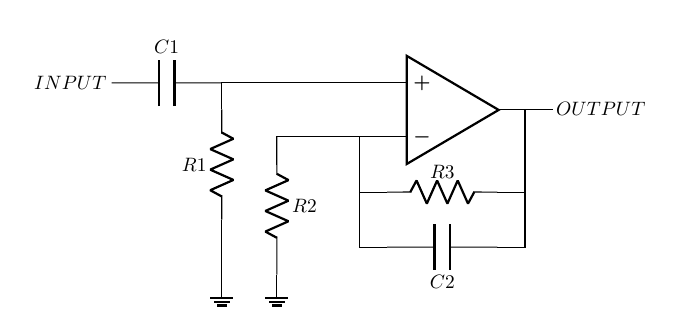
\begin{tikzpicture}[scale=0.7, transform shape]
	% Paths, nodes and wires:
	\node[op amp, yscale=-1] at (2.19, 6.49){};
	\draw (1, 5) to[american resistor] (3, 5);
	\draw (1, 4) to[capacitor] (3, 4);
	\draw (3, 4) -- (3.5, 4) -| (3.5, 5);
	\draw (1, 4) -- (0.5, 4) -| (0.5, 5);
	\draw (1, 5) -- (0.5, 5);
	\draw (-1, 6) to[american resistor] (-1, 3.5);
	\draw (-1, 5.5) -- (-1, 6) -- (0.5, 6);
	\node[ground] at (-1, 3.5){};
	\node[ground] at (-2, 3.5){};
	\draw (-2, 3.5) -| (-2, 4.5);
	\draw (1, 6.98) -| (-2, 6.5);
	\draw (-2, 6.5) to[american resistor] (-2, 4.5);
	\draw (-2, 6.98) to[capacitor] (-4, 6.98);
	\draw (3.5, 6.49) -| (4, 6.5);
	\draw (3.38, 6.49) -| (3.5, 5.25);
	\draw (1, 6) -- (0.5, 6) -| (0.5, 5.25);
	\draw (3, 5) -| (3.5, 5.25);
	\draw (0.5, 4.75) -- (0.5, 5.25);
	\node[shape=rectangle, minimum width=1.215cm, minimum height=0.715cm](R1) at (-3, 7.625){} node[anchor=center] at (R1.text){$C1$};
	\node[shape=rectangle, minimum width=1.215cm, minimum height=0.715cm](N1) at (-2.5, 5.5){} node[anchor=center] at (N1.text){$R1$};
	\node[shape=rectangle, minimum width=1.215cm, minimum height=0.715cm](N2) at (-0.5, 4.75){} node[anchor=center] at (N2.text){$R2$};
	\node[shape=rectangle, minimum width=1.215cm, minimum height=0.715cm](N3) at (2, 5.375){} node[anchor=center] at (N3.text){$R3$};
	\node[shape=rectangle, minimum width=1.215cm, minimum height=0.715cm](N4) at (2, 3.375){} node[anchor=center] at (N4.text){$C2$};
	\node[shape=rectangle, minimum width=1.465cm, minimum height=0.715cm](N5) at (-4.75, 6.98){} node[anchor=center] at (N5.text){$INPUT$};
	\node[shape=rectangle, minimum width=1.715cm, minimum height=0.715cm](N6) at (4.875, 6.5){} node[anchor=center] at (N6.text){$OUTPUT$};
    
\end{tikzpicture}
}
\caption{Schemat pierwszego filtru typu BANDPASS}
\end{figure}



\vspace{-13pt}
\subsection{Wstępne obliczenia}
\noindent Pierwszy filtr pasmowo-przepustowy posiada dwa bieguny (spadek ch. częstotliwościowej 20db/dec dla filtrowanych częstotliwości), jeden biegun związany jest ze stałą czasową związaną z $C_1$ oraz $R_1$ na wejściu nieodwracającym wzmacniacza operacyjnego. Drugi biegun związany jest z komponentami $R_3$ oraz $C_2$. Wartości idealne zostały podane w treści instrukcji do projektu.

\begin{table}[h]
    \centering
    \begin{tabular}{|c|c|c|c|c|c|}
    \hline
                     & $R_1$   & $R_2$ & $R_3$ & $C_1$ & $C_2$  \\
    \hline
    Idealna wartość: & 330k    & 1k    &  100k &  1uF  & 3.3nF  \\
    \hline
    Użyta wartość:   & 326k    & 984    &  99k &  0.9uF  & 3.1nF  \\
    \hline
    \end{tabular}
    \caption{Wartości komponentów dla pierwszego filtru}
\end{table}
\noindent Obliczenia dla częstotliwości granicznych:
\begin{align*}
    f_d &= \frac{1}{2\pi C_1R_1} = \frac{1}{2\pi * 1u  * 330k} = 0.4822 \text{ Hz} \approx 0.5 \text{ Hz} \\
    f_g &= \frac{1}{2\pi C_2 R_3} = \frac{1}{2\pi * 3.3n  * 100k} = 488.28 \text{ Hz} \approx 500 \text{ Hz}
    \\
\end{align*}

Obliczone teoretycznie wartości zgadzają się z symulacjami wykonanymi w środowisku LTspice.

\newpage
\subsection{Przebiegi uzyskane w czasie symulacji oraz pomiarów}

\noindent Poniżej przedstawiono symulowaną charakterystykę filtru z zaznaczonymi punktami -3db.
\begin{figure}[h]
    \centering
    \includegraphics[width=1\linewidth]{proj//png/BP1_sim.png}
    \vspace{-25pt}
    \caption{Symulowana charakterystyka filtru BP1}
\end{figure}

Celem porównania charakterystyki teoretycznej z praktyczną implementacją układu na płytce prototypowej opracowano skrypt w języku Python, który porównuje wyniki z symulacji (plik .txt wyeksportowany z LTspice) z uzyskanymi pomiarami (amplitudy oraz częstotliwość wyjściowego sygnału). Uzyskane wyniki przedstawiono poniżej:

\begin{Verbatim}[frame=single]
 SYMULACJA:
Maksymalne wzmocnienie  40.07  dB
Punkty 3dB: ['0.486 Hz', '477.0 Hz']
 POMIARY:
Maksymalne wzmocnienie:  40.67  dB
Punkty 3dB: ['0.512 Hz', '493.0 Hz']
\end{Verbatim}

\begin{figure}[h]
    \centering
    \includegraphics[width=1\linewidth]{proj//png/BP1_porownanie.png}
    \vspace{-25pt}
    \caption{Porównanie charakterystyk teoretycznych z wykonanymi pomiarami}
\end{figure}

\noindent Wnioski zawarte zostały w dziale \textbf{Wnioski} znajdującym się pod koniec sprawozdania.


% ===============           BP 2
\clearpage
\section{Konstrukcja drugiego filtru pasmowo przepustowego}

Drugi filtr pasmowo-przepustowy typu Butterworth'a miał posiadać pasmo przepustowe w zakresie od 1 Hz do 400 Hz.

\begin{figure}[h]
\centering
\resizebox{0.99\linewidth}{!}{

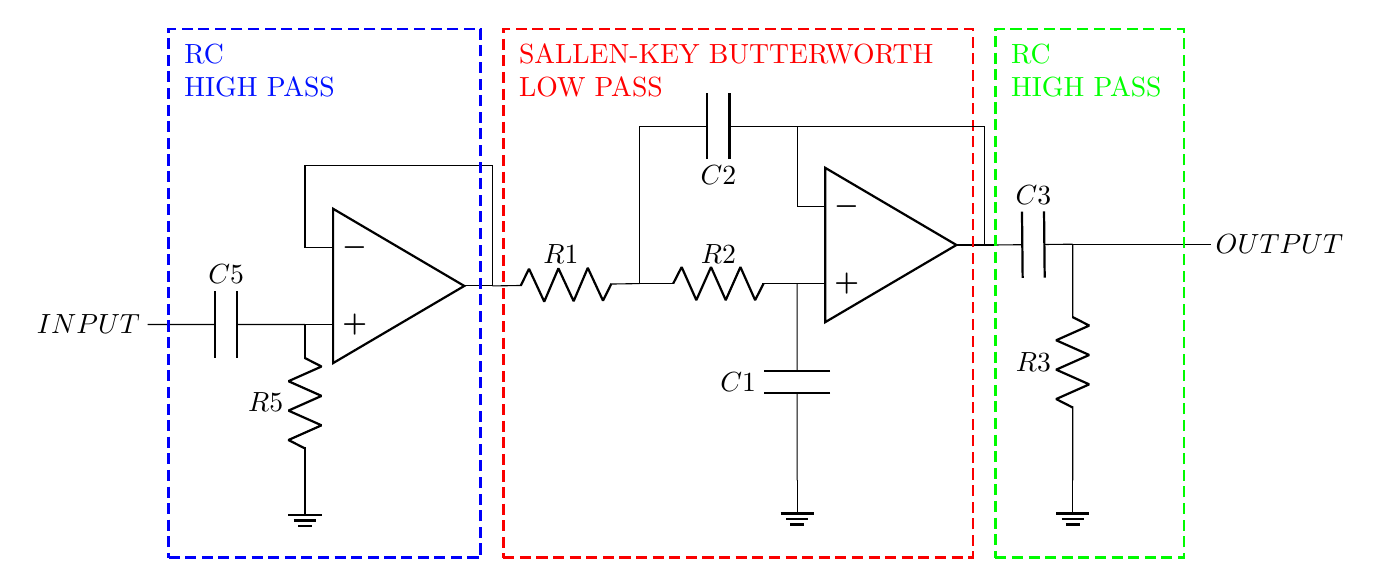
\begin{tikzpicture}[scale=1, transform shape]

	% Paths, nodes and wires:
	\node[op amp] at (-0.06, 7.47){};
	\draw (-1.25, 6.98) to[american resistor] (-1.25, 4.98);
	\draw (-1.25, 6.98) to[capacitor] (-3.25, 6.98);
	\node[shape=rectangle, minimum width=1.215cm, minimum height=0.715cm](R1) at (-2.25, 7.625){} node[anchor=center] at (R1.text){$C5$};
	\node[shape=rectangle, minimum width=1.215cm, minimum height=0.715cm](N1) at (-1.75, 6){} node[anchor=center] at (N1.text){$R5$};
	\node[shape=rectangle, minimum width=1.465cm, minimum height=0.715cm](N2) at (-4, 6.98){} node[anchor=center] at (N2.text){$INPUT$};
	\node[shape=rectangle, minimum width=1.715cm, minimum height=0.715cm](N3) at (11.125, 8){} node[anchor=center] at (N3.text){$OUTPUT$};
	\draw (1.13, 7.47) to[american resistor] (3, 7.5);
	\draw (3, 7.5) to[american resistor] (5, 7.5);
	\draw (5, 7.5) to[capacitor] (5, 5);
	\node[op amp] at (6.19, 7.99){};
	\node[ground] at (-1.25, 4.98){};
	\node[ground] at (5, 5){};
	\draw (7.5, 7.99) to[capacitor] (8.5, 8);
	\draw (8.5, 8) -| (10.25, 8);
	\draw (8.5, 8) to[american resistor] (8.5, 5);
	\node[ground] at (8.5, 5){};
	\draw (5, 9.5) to[capacitor] (3, 9.5);
	\node[shape=rectangle, minimum width=1.215cm, minimum height=0.715cm](N4) at (2, 7.875){} node[anchor=center] at (N4.text){$R1$};
	\node[shape=rectangle, minimum width=1.215cm, minimum height=0.715cm](N5) at (4, 7.875){} node[anchor=center] at (N5.text){$R2$};
	\node[shape=rectangle, minimum width=1.215cm, minimum height=0.715cm](N6) at (4.25, 6.25){} node[anchor=center] at (N6.text){$C1$};
	\node[shape=rectangle, minimum width=1.215cm, minimum height=0.715cm](N7) at (4, 8.875){} node[anchor=center] at (N7.text){$C2$};
	\node[shape=rectangle, minimum width=1.215cm, minimum height=0.715cm](N8) at (8, 8.625){} node[anchor=center] at (N8.text){$C3$};
	\node[shape=rectangle, minimum width=1.215cm, minimum height=0.715cm](N9) at (8, 6.5){} node[anchor=center] at (N9.text){$R3$};
	\draw (-1.25, 7.96) -- (-1.25, 9) -- (1, 9) -| (1.13, 7.47);
	\node[shape=rectangle, draw={rgb,255:red,0;green,0;blue,250}, line width=1pt, dash pattern={on 4pt off 2pt}, minimum width=3.965cm, minimum height=6.715cm] at (-1, 7.375){};
	\node[shape=rectangle, draw={rgb,255:red,250;green,0;blue,0}, line width=1pt, dash pattern={on 4pt off 2pt}, minimum width=5.965cm, minimum height=6.715cm] at (4.25, 7.375){};
	\node[shape=rectangle, draw={rgb,255:red,0;green,250;blue,0}, line width=1pt, dash pattern={on 4pt off 2pt}, minimum width=2.397cm, minimum height=6.715cm] at (8.716, 7.375){};
	\node[shape=rectangle, minimum width=3.965cm, minimum height=1.215cm] at (-1, 10.125){} node[anchor=north west, align=left, text width=3.577cm, inner sep=6pt] at (-3, 10.75){\textcolor{rgb,255:red,0;green,17;blue,255}{RC\\HIGH PASS}};
	\node[shape=rectangle, minimum width=6.215cm, minimum height=1.215cm] at (4.375, 10.125){} node[anchor=north west, align=left, text width=5.827cm, inner sep=6pt] at (1.25, 10.75){\textcolor{rgb,255:red,255;green,0;blue,0}{SALLEN-KEY BUTTERWORTH\\LOW PASS}};
	\node[shape=rectangle, minimum width=2.465cm, minimum height=1.215cm] at (8.75, 10.125){} node[anchor=north west, align=left, text width=2.077cm, inner sep=6pt] at (7.5, 10.75){\textcolor{rgb,255:red,0;green,255;blue,0}{RC\\HIGH PASS}};
	\draw (5, 8.48) -| (5, 9.5) -- (7.25, 9.5) -| (7.38, 7.99) -| (7.5, 7.99);
	\draw (3, 7.5) -| (3, 9.5);


\end{tikzpicture}
}
\caption{Schemat drugiego filtru typu BANDPASS}
\end{figure}

Filtr składa się z dwóch części górno-przepustowych (niebieska oraz zielona) realizowanych za pomocą (buforowanych) pasywnych filtrów RC oraz części dolnoprzepustowej (czerwona) drugiego rzędu typu Sallen-Key.



\subsection{Obliczenia oraz symulacje}

\noindent Poniżej zamieszczono tabelę użytych komponentów:\footnote{Skróty użyte w tabeli: I - ideal: U - used}

\begin{table}[h]
    \centering
    \resizebox{0.5\textwidth}{!}{ % skalowanie do szerokości tekstu
    \begin{tabular}{|c|c|c|c|c|c|c|c|c|}
    \hline
     & \textcolor{blue}{R5} & \textcolor{blue}{C5} & \textcolor{green}{R3} & \textcolor{green}{C3} & \textcolor{red}{C1} & \textcolor{red}{C2} & \textcolor{red}{R1} & \textcolor{red}{R2} \\
    \hline
    I: & 160k & 1u & 160k & 1u & 1n & 3n & 165k & 588k \\
    \hline
    U: & 163k & 0.95u & 162k & 0.90u & 0.80n & 3.05n & 165k & 558k \\
    \hline
    \end{tabular}
    }
    \caption{Wartości komponentów dla drugiego filtru}
\end{table}

\noindent Do obliczenia wkładu części dolnoprzepustowych (zakładamy: $C_5 = C_3$ oraz $R_5 = R_3$) użyto poniższych równań:
\vspace{-7pt}
\begin{align*}
    f_d &= \frac{1}{2\pi C_5R_5} = \frac{1}{2\pi * 1u  * 160k} = 0.9947 \text{ Hz} \approx 1 \text{ Hz} \\
\end{align*}

\vspace{-7pt}
\noindent Do obliczenia elementów pasywnych dla filtru Sallen-Key użyto równań oraz wyprowadzeń zawartych w \cite{TI-OpAmps} na stronach 13-17 oraz Tab. 16-5. Na podstawie zawartych tam wzorów utworzono w serwisie Desmos kalkulator elementów pasywnych\footnote{\href{https://www.desmos.com/calculator/qhmg8bp49s?lang=pl}{EAM second order filter calculator by kszdom}}.

\vspace{10pt}

Filtr jest czwartego rzędu (spadek 40db/dec), dlatego przy rozważaniu punktów częstotliwości granicznych filtru rozważa się punkty 6db a nie 3db.

\begin{figure}[h]
    \centering
    \includegraphics[width=1\linewidth]{proj/png/BP2_sim.png}
    \vspace{-25pt}
    \caption{Symulowana charakterystyka filtru BP2}
\end{figure}




\newpage
\subsection{Porównanie charakterystyki teoretycznej z praktyczną}

Tak jak w przypadku poprzedniego filtru zastosowano skrypt w języku Python celem porównania wynikó symulacji z praktyczną implementacją filtru. Wyniki przedstawiono poniżej:

\begin{Verbatim}[frame=single]
 SYMULACJA:
Wartość szczytowa symulacji:  -0.0702  dB
6 dB points: ['0.997 Hz', '397.0 Hz']
 POMIARY:
Wartość szczytowa pomiarów:  0.2848  dB
6 dB points: ['1.01 Hz', '408.0 Hz']
\end{Verbatim}

\vspace{-10pt}

\begin{figure}[h]
    \centering
    \includegraphics[width=1\linewidth]{proj//png/BP2_porownanie.png}
    \vspace{-25pt}
    \caption{Porównanie charakterystyk teoretycznych z wykonanymi pomiarami}
\end{figure}


\noindent Pomiary wykonywano dla wejściowego sygnału sinusoidalnego o amplitudzie między-szczytowej $3 V_{pp}$.











% ===============           ROZDZIAL 3 
\clearpage
\section{Konstrukcja filtru typu notch}

Rejestracja biosygnałów powyższymi filtrami cechuje się pasmem sygnału z zakresie od 1Hz do 100Hz. Niestety w powyższym zakresie znajduje się częstotliwość linii energetycznej (50Hz), co powoduje duże problemy związane z EMI\footnote{EMI: Electromagnetic Interference (tj. zakłócenia elektromagnetyczne)} dla tej częstotliwości. Należy więc zastosować filtr wysoce selektywny typu "notch" wycinający zakłócenia z linii energetycznej.
\vspace{-5pt}
\subsection{Wybrana architektura filtru notch}

\subsection{Filtr notch typu TWIN-T}

Istnieje wiele architektur dla filtrów typu "notch". Jeden z najpopularniejszych to filtr typu TWIN-T przedstawiony na poniższym schemacie. Niestety powyższy filtr jest czuły na rozrzut komponentów, oraz nie jest możliwa regulacja wycinanej częstotliwości.
\vspace{-10pt}
\begin{figure}[h]
\centering
\resizebox{0.75\linewidth}{!}{
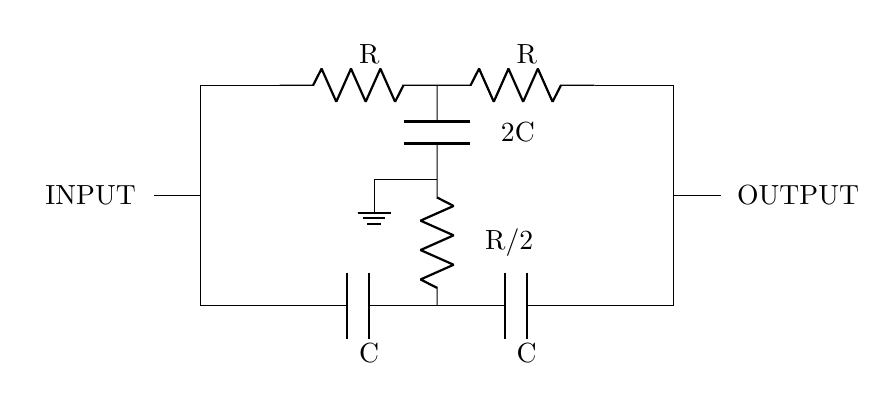
\begin{tikzpicture}
	% Paths, nodes and wires:
	\draw (3, 11) to[american resistor] (5, 11);
	\draw (5, 11) to[american resistor] (7, 11);
	\draw (3, 8.2) to[capacitor] (5, 8.2);
	\draw (5, 8.2) to[american resistor] (5, 9.8);
	\draw (5, 11) to[capacitor] (5, 9.8);
	\draw (7, 11) -- (8, 11) -| (8, 8.2) -- (7, 8.2);
	\draw (3, 8.2) -- (2, 8.2) -- (2, 11) -- (3, 11);
	\draw (5, 9.8) -- (4.2, 9.8);
	\node[ground] at (4.2, 9.8){};
	\node[ground] at (4.2, 9.8){};
	\node[ground] at (4.2, 9.8){};
	\draw (2, 9.6) -- (1.4, 9.6);
	\draw (8, 9.6) -- (8.6, 9.6);
	\node[shape=rectangle, minimum width=1.565cm, minimum height=0.365cm] at (9.4, 9.6){} node[anchor=center, align=center, text width=1.177cm, inner sep=6pt] at (9.4, 9.6){OUTPUT};
	\node[shape=rectangle, minimum width=1.565cm, minimum height=0.365cm] at (0.6, 9.6){} node[anchor=center, align=center, text width=1.177cm, inner sep=6pt] at (0.6, 9.6){INPUT};
	\node[shape=rectangle, minimum width=0.365cm, minimum height=0.365cm] at (4, 11.4){} node[anchor=center, align=center, text width=-0.023cm, inner sep=6pt] at (4, 11.4){R};
	\node[shape=rectangle, minimum width=0.365cm, minimum height=0.365cm] at (6, 11.4){} node[anchor=center, align=center, text width=-0.023cm, inner sep=6pt] at (6, 11.4){R};
	\node[shape=rectangle, minimum width=0.365cm, minimum height=0.365cm] at (5.6, 9){} node[anchor=center, align=center, text width=-0.023cm, inner sep=6pt] at (5.6, 9){R/2};
	\node[shape=rectangle, minimum width=0.365cm, minimum height=0.365cm] at (5.8, 10.4){} node[anchor=center, align=center, text width=-0.023cm, inner sep=6pt] at (5.8, 10.4){2C};
	\draw (5, 8.2) to[capacitor] (7, 8.2);
	\node[shape=rectangle, minimum width=0.365cm, minimum height=0.365cm] at (6, 7.6){} node[anchor=center, align=center, text width=-0.023cm, inner sep=6pt] at (6, 7.6){C};
	\node[shape=rectangle, minimum width=0.365cm, minimum height=0.365cm] at (4, 7.6){} node[anchor=center, align=center, text width=-0.023cm, inner sep=6pt] at (4, 7.6){C};
\end{tikzpicture}
}
\vspace{-10pt}
\caption{Schemat filtru notch typu TWIN-T}
\end{figure}
\vspace{-15pt}
\subsection{Filtr notch typu FLIEGE}

Poniżej przedstawiono architektura opisaną w \cite{HighSpeedNotch}, typu FLIEGE. Posiada trzy zalety w stosunku do filtrów typu TWIN-T:

\begin{itemize}
    \item Do jej budowy potrzebne są tylko cztery precyzyjne komponenty (CF1, CF2, RF1, RF2).
    \item Dobroć filtru może być ustawiona za pomocą rezystorów RQ.
    \item Wycinana częstotliwość może być dostrajana w niewielkim zakresie potencjometrem RP, na koszt tłumienia.
\end{itemize}

\begin{figure}[h]
\centering
\resizebox{0.8\linewidth}{!}{

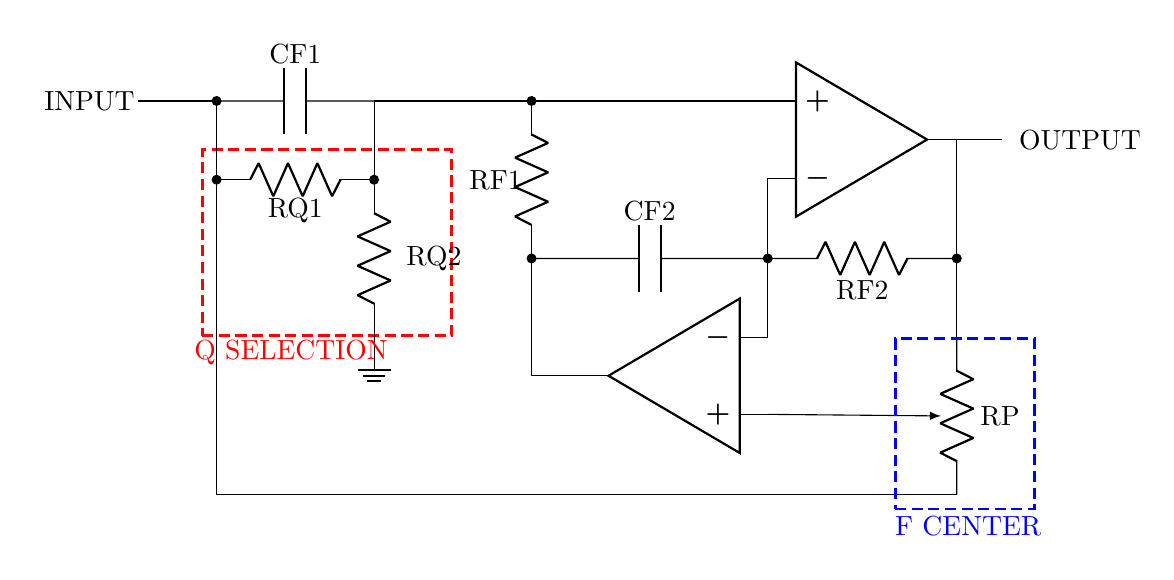
\begin{tikzpicture}
	% Paths, nodes and wires:
	\node[shape=rectangle, draw={rgb,255:red,255;green,0;blue,0}, line width=1pt, dash pattern={on 4pt off 2pt}, minimum width=3.165cm, minimum height=2.365cm] at (1.4, 9.2){};
	\draw (9.38, 10.51) -- (9.98, 10.51);
	\node[shape=rectangle, minimum width=1.565cm, minimum height=0.365cm] at (10.78, 10.51){} node[anchor=center, align=center, text width=1.177cm, inner sep=6pt] at (10.78, 10.51){OUTPUT};
	\node[shape=rectangle, minimum width=1.365cm, minimum height=0.365cm] at (-1.7, 11){} node[anchor=center, align=center, text width=0.977cm, inner sep=6pt] at (-1.7, 11){INPUT};
	\draw (0, 11) to[capacitor] (2, 11);
	\draw (0, 10) to[american resistor] (2, 10);
	\draw (2, 10) to[american resistor] (2, 8);
	\node[ground] at (2, 8){};
	\draw (0, 10) -| (0, 11);
	\draw (2, 10) -| (2, 11);
	\draw (2, 11) -- (4, 11);
	\draw (4, 11) to[american resistor] (4, 9);
	\node[op amp, yscale=-1] at (8.19, 10.51){};
	\draw (4, 11) -- (6, 11);
	\node[op amp, xscale=-1] at (5.81, 7.51){};
	\draw (4, 9) to[capacitor] (7, 9);
	\draw (4.62, 7.51) -| (4, 7.6) -| (4, 9);
	\draw (7, 8) -| (7, 9);
	\draw (6, 11) -- (7, 11);
	\draw (7, 9) -- (7, 10.02);
	\draw (9.38, 10.51) -| (9.4, 8);
	\draw (0, 11) -- (-1, 11);
	\draw (9.4, 6) -| (0, 10);
	\node[shape=rectangle, minimum width=1.365cm, minimum height=0.365cm] at (1, 11.6){} node[anchor=center, align=center, text width=0.977cm, inner sep=6pt] at (1, 11.6){CF1};
	\node[shape=rectangle, minimum width=0.365cm, minimum height=0.365cm] at (2.4, 9){} node[anchor=center, align=center, text width=-0.023cm, inner sep=6pt] at (2.4, 9){RQ2};
	\node[shape=rectangle, minimum width=1.365cm, minimum height=0.365cm] at (1, 9.6){} node[anchor=center, align=center, text width=0.977cm, inner sep=6pt] at (1, 9.6){RQ1};
	\node[shape=rectangle, minimum width=1.365cm, minimum height=0.365cm] at (5.5, 9.6){} node[anchor=center, align=center, text width=0.977cm, inner sep=6pt] at (5.5, 9.6){CF2};
	\node[shape=rectangle, minimum width=0.365cm, minimum height=0.365cm] at (3.2, 10){} node[anchor=center, align=center, text width=-0.023cm, inner sep=6pt] at (3.2, 10){RF1};
	\node[shape=rectangle, minimum width=1.065cm, minimum height=0.365cm] at (9.95, 7){} node[anchor=center, align=center, text width=0.677cm, inner sep=6pt] at (9.95, 7){RP};
	\draw (7, 9) to[american resistor] (9.4, 9);
	\draw (9.4, 8) to[american resistor] (9.4, 6);
	\draw[-latex] (7, 7.02) -- (9.2, 7);
	\node[circ] at (7, 9){};
	\node[circ] at (4, 9){};
	\node[circ] at (2, 10){};
	\node[circ] at (0, 11){};
	\node[circ] at (4, 11){};
	\node[circ] at (9.4, 9){};
	\node[circ] at (0, 10){};
	\node[shape=rectangle, minimum width=1.365cm, minimum height=0.365cm] at (8.2, 8.6){} node[anchor=center, align=center, text width=0.977cm, inner sep=6pt] at (8.2, 8.6){RF2};
	\node[shape=rectangle, draw={rgb,255:red,0;green,0;blue,255}, line width=1pt, dash pattern={on 4pt off 2pt}, minimum width=1.765cm, minimum height=2.165cm] at (9.5, 6.9){};
	\node[shape=rectangle, minimum width=3.365cm, minimum height=0.365cm] at (10.1, 5.6){} node[anchor=west, align=left, text width=2.977cm, inner sep=6pt] at (8.4, 5.6){\textcolor{rgb,255:red,0;green,0;blue,255}{F CENTER}};
	\node[shape=rectangle, minimum width=3.365cm, minimum height=0.365cm] at (1.2, 7.8){} node[anchor=west, align=left, text width=2.977cm, inner sep=6pt] at (-0.5, 7.8){\textcolor{rgb,255:red,255;green,0;blue,0}{Q SELECTION}};
\end{tikzpicture}
}
\caption{Schemat filtru notch typu FLIEGE}
\end{figure}




\newpage
\subsection{Dobór komponentów}

Wartości dobrane zostały według wzorów z publikacji \cite{HighSpeedNotch}\footnote{Publiacja dostepna jest pod adresem: \url{https://www.ti.com/lit/an/slyt235/slyt235.pdf}}.
\begin{align*}
    f_c &= \frac{1}{2\pi C_FR_F} = \frac{1}{2\pi * 10n  * 318k} = 50.048 \text{ Hz} \approx 50 \text{ Hz} \\
    Q&= \frac{R_Q}{2*R_F} = \frac{1MEG}{2*318k} = 1.57 \\
\end{align*}

\noindent Poniżej zamieszczono tabelę użytych komponentów:

\begin{table}[h]
    \centering
    \resizebox{0.5\textwidth}{!}{ % skalowanie do szerokości tekstu
    \begin{tabular}{|c|c|c|c|c|c|c|c|c|}
    \hline
     & \textcolor{black}{RF1} & \textcolor{black}{RF2} & \textcolor{black}{CF1} & \textcolor{black}{CF2} & \textcolor{red}{RQ1} & \textcolor{red}{RQ2} & \textcolor{blue}{RP} \\
    \hline
    I: & 318k & 318k & 10n & 10n & 1MEG & 1MEG & 10k \\
    \hline
    U: & 297k & 297k & 10.6n & 10.6n & 1MEG & 1MEG & 10k \\
    \hline
    \end{tabular}
    }
    \caption{Wartości komponentów dla filtru notch}
\end{table}

\subsection{Symulacje dla filtru typu FLIEGE}
Poniżej zamieszczono wyniki symulacji. Symulowano kręcenie potencjometrem w zakresie 8k - 12k.
\vspace{-10pt}
\begin{figure}[h]
    \centering
    \includegraphics[width=1\linewidth]{proj//png/FLIEGE.png}
    \vspace{-25pt}
    \caption{Symulowana charakterystyka dla zaprojektowanego filtru}
\end{figure}

\vspace{-22pt}

\subsection{Porównanie charakterystyki teoretycznej z praktyczną}
\noindent Przed pomiarami dokonano kalibracji: na wejście układu podano sygnał sinusoidalny 50 Hz oraz tak ustawiono potencjometr aby tłumienie sygnału było największe.

\vspace{10pt}

\noindent Niestety zlutowany układ nie tłumił 50Hz dla żadnych ustawień potencjometru. Na wejście podano sinusa o amplitudzie $1V_{pp}$, na wyjściu otrzymano minimalną amplitudę o wartości $920mV$. Zdecydowano się nie umieszczać wyników w sprawozdaniu oraz zaniechać używania filtru NOTCH podczas pomiarów całego toru wzmacniającego.






















% ===============           ROZDZIAL 6 
\newpage
\section{Prezentacja działania wzmacniacza biopotencjałów}

Na płytce prototypowej dolutowano układ PGA204 wraz z elementami pasywnymi - rezystancje wejściowe oraz kondensatory odsprzęgające.

\vspace{10pt}

\noindent Na poniższych zdjęciach widać zlutowany układ oraz zaznaczone poszczególne elementy toru przetwarzania sygnałów:

\begin{figure}[h]
    \centering
    \includegraphics[width=1\linewidth]{proj//png/caly_uklad.png}
    \caption{Zdjęcie oraz pokolorowany schemat układu}
\end{figure}


\subsection{Weryfikacja działania układu PGA204}

Na wejście układu PGA podano przebieg sinusoidalny o częstotliwości 100Hz oraz amplitudzie $10mV_{pp}$. Badano przebiegi na wyjściu celem weryfikacji cyfrowego ustawienia wzmocnienia.

\begin{figure}[h]
    \centering
    \includegraphics[width=1\linewidth]{proj/png/PGA1.png}
\end{figure}

\vspace{-23pt}

\begin{figure}[h]
    \centering
    \includegraphics[width=1\linewidth]{proj/png/PGA2.png}
    \caption{Pomiary przebiegów dla różnego ustawienia amplitud.}
\end{figure}

\begin{Verbatim}[frame=single]
Pomiar układu PGA dla ustawienń:
A0 = 0 oraz A1 = 1

amplitude ch1:  0.194
amplitude ch2:  0.0148
gain:  13.108108108108109
\end{Verbatim}
\begin{Verbatim}[frame=single]
Pomiar układu PGA dla ustawienń:
A0 = 1 oraz A1 = 1

amplitude ch1:  15.0
amplitude ch2:  0.013999999999999999
gain:  1071.4285714285716
\end{Verbatim}



\subsection{Pomiary EKG}

Po podłączeniu trzech elektrod:
\begin{itemize}
    \item elektroda czarna: BIAS, podpięta do prawej kostki,
    \item elektroda czerwona: IN+, podpieta do lewej kostki
    \item elektroda niebieskia: IN-, podpięta do prawej ręki,
\end{itemize}
dokonano pomiarów na wyjściu toru pomiarowego.

Niestety przez brak układu filtrującego typu NOTCH na wyjściu dało się zauważyć piękną sinusoidę o częstotliwości 50Hz. 



\begin{figure}[h]
    \centering
    \includegraphics[width=1\linewidth]{proj/png/EKG2.png}
    \caption{Zbliżenie na uzyskany przebieg - widoczne zakłócenia sieciowe o częstotliwości 50Hz}
\end{figure}

Jednakże po zebraniu próbek z dłuższej ilości czasu zauważono okresowo występujące piki odpowiadające sygnałom EKG - po dokonaniu uśredniania 4 próbek udało się w domenie cyfrowej odfiltrować zakłócenia sieciowe. Tętno obliczono jako wartość czasu między dwoma pikami. Uzyskane przebiegi przedstawiono na poniższym wykresie.


\begin{figure}[h]
    \centering
    \includegraphics[width=1\linewidth]{proj/png/EKGpiekne.png}
    \caption{Uzyskane przebiegi oraz pomiar tętna}
\end{figure}




% ===============           WNIOSKI 
\clearpage
\section{Wnioski}

\subsection{Konstrukcja pierwszego filtru pasmowo przepustowego}
\noindent Skonstruowany układ praktycznie nie różni się od symulowanego.
Ewentualne rozbieżności pomiędzy symulacjami a pomiarami wynikają z:
\begin{itemize}
    \item nie-idealności użytych komponentów (nieznaczne
    \newline przesunięcie się punktów -3db oraz zwiększenie \newline wzmocnienia o 0.5dB),
    \item nie-idealności, efektów wyższego rzędu (zera i bieguny niedominujące nieopisane w nocie katalogowej wzmacniacza TL082) co skutkuje rozbieżnością pomiędzy pomiarami a symulacją pod koniec charakterystyki (od 5kHz w górę);
\end{itemize}

\subsection{Konstrukcja drugiego filtru pasmowo przepustowego}
\noindent Skonstruowany układ praktycznie nie różni się od symulowanego. Dolna wartość częstotliwości dla wzmocnienia -6db wynosi 1.01 Hz co jest 0.01Hz oddalone od specyfikowanej. Wartość górna "przesunęła" się o 8Hz w górę, co nie wpływa na działanie układu (400Hz). Układ działa zgodnie z założoną specyfikacją.


\subsection{Konstrukcja filtru typu notch}
Projekt samego filtru notch nie był skomplikowany - łatwo było wyznaczyć oraz zasymować działanie układu. Szczególnie zważając na istnienie cytowanej noty aplikacyjnej \cite{HighSpeedNotch}. Lutowanie jednak, zajęło bardzo dużą ilość czasu, po których filtr nie działał (4 zajęcia laboratoryjne)- czas ten można było przeznaczyć na coś innego.

\begin{figure}[h]
    \centering
    \includegraphics[width=0.75\linewidth]{proj/png/50Hz mem2.png}
    \caption{Humorystyczna grafika przedstawiająca problemy z zakłóceniami sieciowymi w układach biomedycznych}
\end{figure}


\subsection{Weryfikacja działania układu PGA204}
Układ PGA204 zamontowano poprawnie. Wzmocnienie dla testowanych ustawień jest zgodne z oczekiwanym (do wartości amplitudy brano skrajne wartości napieć - na sygnał nałożony jest szum który powoduje zawyżone wyniki).
\begin{table}[h]
    \centering
    \begin{tabular}{c|c|c|c}
        Wzmocnienie & Wzmocnienie  &  &  \\
         oczekiwane & uzyskane      & $A_1$ & $A_0$ \\
        \hline
        10 & 13 & 0 & 1 \\
        1000 & 1071 & 1 & 1 \\
    \end{tabular}
    \caption{Uzyskane wzmocnienia dla różnych ustawień PGA204}
\end{table}


\subsection{Pomiary EKG}
Brak filtra NOTCH, wycinający zakłócenia sieciowe okazał sie być o wiele większym problemem niż zakładano, na szczęście analiza sygnałów z EKG została uratowana poprzez zastosowanie DSP oraz funkcji uśredniania dla okna o szerokości 4 próbek - uzyskano wtedy przebieg EKG, który mógł być poddany dalszej analizie. Udało się zmierzyć tętno na poziomie 70.6 BPM, co uznaje się za odpowiednie dla tętna spoczynkowego - badana osoba siedziała wówczas na stanowisku w laboratorium.

\subsection{Wnioski ogólne}
Lepszym pomysłem byłoby wykonanie projektu płytki prototypowej z każdą częścią układu pomiarowego tak, aby możliwe było dowolne rozłączanie i testowanie każdego z filtrów z osobna; oraz zamówienie jest np. z JLCPCB aniżeli wykonywanie układu na płytce typu \textit{perfboard}. Końcowo zaoszczędziłoby to czas oraz wyglądało o wiele estetyczniej.



\bibliographystyle{plain}
\bibliography{references}





\end{document}